% Hier folgt der Inhalt des Abschnitts "Ergebnisse und Bewertung".
\section{Ergebnisse und Bewertung}

In diesem Abschnitt werden die erzielten Ergebnisse des Projekts beschrieben und kritisch bewertet. Der Fokus liegt auf der funktionalen Umsetzung, der Leistungsbewertung des Systems und einer Analyse der Stärken und Schwächen.

\subsection{Funktionale Ergebnisse}

Das Projektziel, einen voll funktionsfähigen Prototypen für einen smarten Cocktailautomaten zu entwickeln, wurde erfolgreich erreicht. Die wesentlichen funktionalen Anforderungen konnten umgesetzt werden:

\begin{itemize}
  \item \textbf{Automatisierte Cocktailzubereitung:} Die Hardware steuert präzise die Pumpen und Motoren, um Zutaten gemäß den Rezeptvorgaben abzugeben.
  \item \textbf{Mobile App:} Benutzer können über eine intuitive App Rezepte erstellen, verwalten und Bestellungen auslösen.
  \item \textbf{Backend-Integration:} Das Backend verarbeitet Bestellungen zuverlässig, synchronisiert Benutzerdaten und leitet Steuerbefehle an die Hardware weiter.
\end{itemize}

Die abschließenden Integrationstests zeigten, dass das Gesamtsystem von der Rezeptbestellung in der App bis zur Zubereitung durch die Hardware stabil funktioniert.

\subsection{Lasttestergebnisse und Analyse}

Zur Bewertung der Performance und Skalierbarkeit des Systems wurden umfassende Lasttests mit dem Tool \texttt{k6} durchgeführt. Diese Tests simulierten eine Vielzahl gleichzeitiger Benutzeranfragen, um Engpässe und Optimierungspotenziale zu identifizieren. Die wichtigsten Ergebnisse sind im Folgenden zusammengefasst.

\subsubsection*{Wichtige Metriken}
\begin{itemize}
    \item \textbf{Gesamtanfragen:} 16.506
    \item \textbf{Fehlerrate:} 0,08\% (14 fehlgeschlagene Anfragen)
    \item \textbf{Durchschnittliche Antwortzeit:} 274,48 ms
    \item \textbf{Maximale Antwortzeit:} 282.415,99 ms
    \item \textbf{90. Perzentil der Antwortzeit:} 78,66 ms
    \item \textbf{95. Perzentil der Antwortzeit:} 121,84 ms
\end{itemize}

\subsubsection*{Antwortzeiten pro Endpunkt}

Die Antwortzeiten für spezifische API-Endpunkte zeigen deutliche Unterschiede, die auf unterschiedliche Verarbeitungskomplexität hinweisen. Die wichtigsten Werte sind in Tabelle \ref{tab:response_times} dargestellt.

\begin{table}[h!]
    \centering
    \begin{tabular}{|l|c|c|c|c|}
        \hline
        \textbf{Endpunkt} & \textbf{Durchschnitt (ms)} & \textbf{Median (ms)} & \textbf{90. Perzentil (ms)} & \textbf{Max (ms)} \\
        \hline
        Registrierung & 145,60 & 102,71 & 219,24 & 1.224,99 \\
        Login & 155,91 & 102,52 & 283,80 & 1.530,32 \\
        Rezept anlegen & 136,99 & 19,10 & 42,42 & 282.282,60 \\
        Slot setzen & 1.341,94 & 23,35 & 79,70 & 282.292,87 \\
        „Get Slots“ & 64,93 & 48,97 & 112,32 & 355,33 \\
        „Get Favorites“ & 29,59 & 20,02 & 51,68 & 227,09 \\
        „Create Drink“ & 588,13 & 19,39 & 52,83 & 282.275,99 \\
        \hline
    \end{tabular}
    \caption{Antwortzeiten pro Endpunkt}
    \label{tab:response_times}
\end{table}

\subsubsection*{Visualisierung der Antwortzeiten}

\begin{figure}[h!]
    \centering
    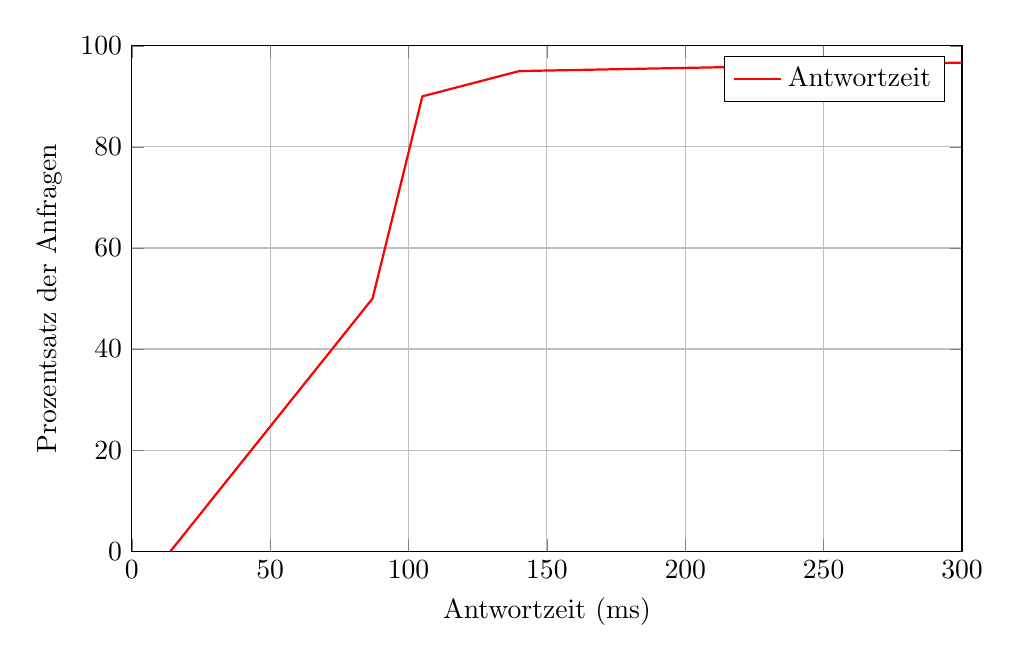
\begin{tikzpicture}
        \begin{axis}[
            width=\textwidth,
            height=8cm,
            xlabel={Antwortzeit (ms)},
            ylabel={Prozentsatz der Anfragen},
            ymin=0, ymax=100,
            xmin=0, xmax=300,
            xtick={0,50,100,150,200,250,300},
            ytick={0,20,40,60,80,100},
            grid=both,
            ]
            \addplot[red, thick] coordinates {
                (14, 0) (87, 50) (105, 90) (140, 95) (522, 99) (644, 100)
            };
            \addlegendentry{Antwortzeit}
        \end{axis}
    \end{tikzpicture}
    \caption{Verteilung der Antwortzeiten}
    \label{fig:response_time_distribution}
\end{figure}

\subsubsection*{Erfolgsquoten der API-Endpunkte}

Die Erfolgsquoten einzelner Endpunkte zeigen, dass die meisten Anfragen erfolgreich waren, jedoch bei einigen spezifischen Funktionen wie der Slot-Registrierung Verbesserungspotenzial besteht (siehe Abbildung \ref{fig:success_rates}).

\begin{figure}[h!]
    \centering
    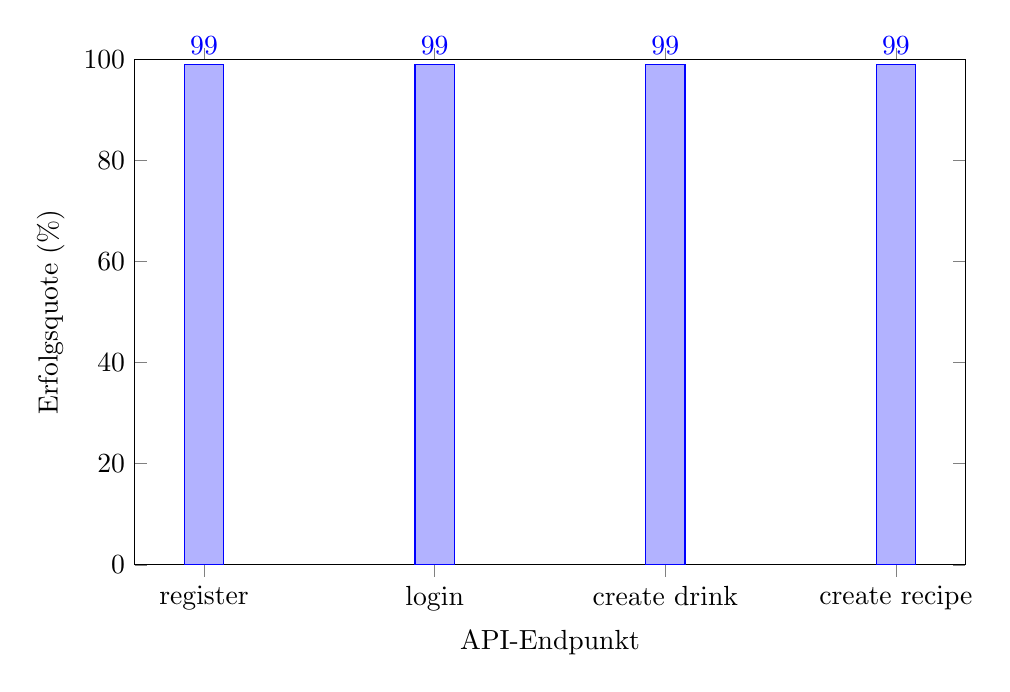
\begin{tikzpicture}
        \begin{axis}[
            ybar,
            width=\textwidth,
            height=8cm,
            xlabel={API-Endpunkt},
            ylabel={Erfolgsquote (\%)},
            ymin=0, ymax=100,
            symbolic x coords={register, login, create drink, create recipe},
            xtick=data,
            bar width=0.5cm,
            nodes near coords,
            nodes near coords align={vertical},
            ]
            \addplot coordinates {(register, 99) (login, 99) (create drink, 99) (create recipe, 99)};
        \end{axis}
    \end{tikzpicture}
    \caption{Erfolgsquoten der API-Endpunkte}
    \label{fig:success_rates}
\end{figure}

\subsubsection*{Zusammenfassung der Ergebnisse}

Die Tests haben gezeigt, dass das System in einer Live-Umgebung grundsätzlich stabil arbeitet. Allerdings wurden Skalierungsprobleme bei Websocket-Verbindungen identifiziert, die durch eine zentrale Verwaltung oder eine konsistente Lastverteilung gelöst werden könnten. Die meisten API-Endpunkte zeigten zufriedenstellende Antwortzeiten und Erfolgsquoten. Die Schwachstellen bieten jedoch Anknüpfungspunkte für zukünftige Optimierungen.

\subsection{Stärken und Schwächen}

\subsubsection*{Stärken}

Das Projekt weist folgende Stärken auf:
\begin{itemize}
  \item \textbf{Benutzerfreundlichkeit:} Die App bietet eine intuitive Benutzeroberfläche und ermöglicht eine einfache Verwaltung von Rezepten und Geräten.
  \item \textbf{Technische Umsetzung:} Die Kombination aus App, Backend und Hardware zeigt das Potenzial von IoT-Technologien in Smart-Home-Umgebungen.
  \item \textbf{Modularität:} Die Architektur des Systems ermöglicht zukünftige Erweiterungen, z. B. die Integration zusätzlicher Geräte oder neue Funktionen.
\end{itemize}

\subsubsection*{Schwächen}

Einige Schwächen des aktuellen Prototyps wurden identifiziert:
\begin{itemize}
  \item \textbf{Skalierbarkeit:} Die Verwaltung von Websocket-Verbindungen in einer containerisierten Umgebung führte bei hoher Last zu Problemen.
  \item \textbf{Fehlende Tests:} Es wurden keine umfassenden automatisierten Tests für die einzelnen Systemkomponenten implementiert.
  \item \textbf{Hardware:} Obwohl die Hardware zuverlässig arbeitet, könnten Optimierungen in der Dosiergenauigkeit und Stabilität vorgenommen werden.
\end{itemize}

\subsection{Zusammenfassung der Ergebnisse}

Das Projekt hat gezeigt, dass IoT-Technologien erfolgreich zur Automatisierung von Alltagsaufgaben eingesetzt werden können. Die entwickelten Systeme arbeiten zuverlässig und erfüllen die definierten funktionalen Anforderungen. Gleichzeitig wurden Schwächen aufgedeckt, die als Grundlage für zukünftige Optimierungen dienen können.

\subsection{Empfehlungen}

Auf Basis der Testergebnisse und identifizierten Schwächen werden folgende Maßnahmen für zukünftige Verbesserungen empfohlen:
\begin{itemize}
  \item \textbf{Optimierung der Skalierung:} Einführung eines zentralen Websocket-Servers oder konsistenter Lastverteilung, um Kommunikationsprobleme bei hoher Last zu beheben.
  \item \textbf{Automatisierte Tests:} Entwicklung und Implementierung umfassender Unit- und Integrationstests.
  \item \textbf{Hardware-Optimierungen:} Verbesserung der Dosiergenauigkeit und Integration zusätzlicher Sensorik zur Überwachung.
\end{itemize}

\section{DUMP}

\subsection{Lasttest Ergebnisse - k6}
% Wir haben einen Lasttest durchgeführt, um die Leistung und Stabilität der API zu bewerten. Die 
% Ergebnisse zeigen, dass die API insgesamt 37.900 Anfragen verarbeiten konnte, wobei 17.097 Anfragen 
% fehlgeschlagen sind. Die durchschnittliche Antwortzeit betrug 66,26 ms, was akzeptabel ist. Die 
% Erfolgsquote für die Benutzerregistrierung und Rezeptverwaltung lag bei 9.

\subsection{Beispiele Plots und Diagramme}

\begin{tikzpicture}[scale=1]
    \begin{axis}[
        axis lines=middle,
        xlabel=,
        ylabel={},
        legend style={
            fill=pag, draw=pag!60, % Red background with black border
            font=\small, % Smaller font size
            inner sep=2pt, % Inner spacing (padding around the text)
            outer sep=1pt  % Outer spacing (margin around the border)
        },
        domain=0:8000,
        xtick=\empty,
        ytick=\empty,
        grid=both,
        grid style={line width=.1pt, draw=gray!10},
        major grid style={line width=.2pt,draw=gray!50},
        minor tick num=5,
        width=1.15*\textwidth,
        height=5cm,
        clip=false,
        ticklabel style={font=\tiny,fill=white},
        xlabel style={at={(ticklabel* cs:1)},anchor=north west},
        ylabel style={at={(ticklabel* cs:1)},anchor=south west},
        ]

        \addplot[color=red1,ultra thick,samples=100]{x};
        \addplot[color=red2,ultra thick,samples=100]{1/x};
        \addplot[color=red3,ultra thick,samples=100]{1/x^2};

        \legend{100, 300, 1000}
    \end{axis}
    \node at (3.5,-0.3) {Velocity};
    \node[rotate=90] at (-0.3,1.65) {Probability};
\end{tikzpicture}

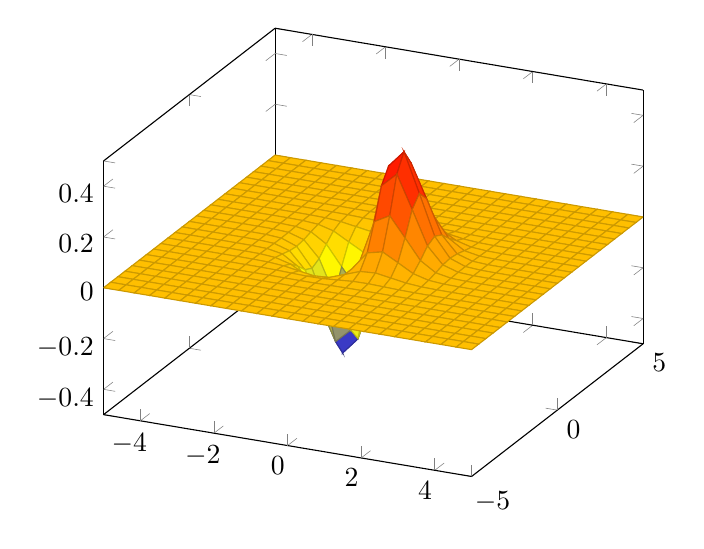
\begin{tikzpicture}
	\begin{axis}
	\addplot3[
			surf,
	]
	{exp(-x^2-y^2)*x};
	\end{axis}
	\end{tikzpicture}

	Plotting from data:

\begin{tikzpicture}
\begin{axis}[
    title={Temperature dependence of CuSO\(_4\cdot\)5H\(_2\)O solubility},
    xlabel={Temperature [\textcelsius]},
    ylabel={Solubility [g per 100 g water]},
    xmin=0, xmax=100,
    ymin=0, ymax=120,
    xtick={0,20,40,60,80,100},
    ytick={0,20,40,60,80,100,120},
    legend style={
        fill=pag, draw=pag!60, % Red background with black border
        font=\small, % Smaller font size
        inner sep=2pt, % Inner spacing (padding around the text)
        outer sep=1pt  % Outer spacing (margin around the border)
    },
    legend pos=north west,
    ymajorgrids=true,
    grid style=dashed,
]

\addplot[color=red2, ultra thick, mark=triangle*]
    coordinates {
    (0,23.1)(10,27.5)(20,32)(30,37.8)(40,44.6)(60,61.8)(80,83.8)(100,114)
    };
    \legend{CuSO\(_4\cdot\)5H\(_2\)O}
    
\end{axis}
\end{tikzpicture}

\paragraph*{Info}
Find more examples here: \url{https://www.overleaf.com/learn/latex/Pgfplots_package}
Or here: \url{https://pgfplots.net/}


\section*{Testergebnisse}

\subsection*{Wichtige Metriken}
\begin{itemize}
    \item \textbf{Gesamtanfragen:} 37.900
    \item \textbf{Fehlerrate:} 45,11\% (17.097 Anfragen fehlgeschlagen)
    \item \textbf{Durchschnittliche Antwortzeit:} 66,26 ms
    \item \textbf{Erfolgsquote Registrierung:} 9\% (927 von 9.475 Iterationen erfolgreich)
    \item \textbf{Erfolgsquote Rezeptverwaltung:} 9\% (926 von 9.475 Iterationen erfolgreich)
\end{itemize}

\subsection*{Antwortzeiten}
\begin{figure}
    \centering
    \begin{tikzpicture}
        \begin{axis}[
            width=\textwidth,
            height=8cm,
            xlabel={Antwortzeit (ms)},
            ylabel={Prozentsatz der Anfragen},
            ymin=0, ymax=100,
            xmin=0, xmax=700,
            xtick={0,100,200,300,400,500,600,700},
            ytick={0,20,40,60,80,100},
            legend style={
                fill=pag, draw=pag!60, % Red background with black border
                font=\small, % Smaller font size
                inner sep=2pt, % Inner spacing (padding around the text)
                outer sep=1pt  % Outer spacing (margin around the border)
            },
            legend pos=north east,
            grid=both,
            ]
            \addplot[red3,ultra thick] coordinates {
                (14, 0) (87, 50) (105, 90) (140, 95) (522, 99) (644, 100)
            };
            \addlegendentry{Antwortzeit}
        \end{axis}
    \end{tikzpicture}
    \caption{Antwortzeiten der API (90. Perzentil: 105 ms, 95. Perzentil: 140 ms)}
    \label{fig:response_time}
\end{figure}

\subsection*{Erfolgsquoten der Checks}
\begin{figure}
    \centering
    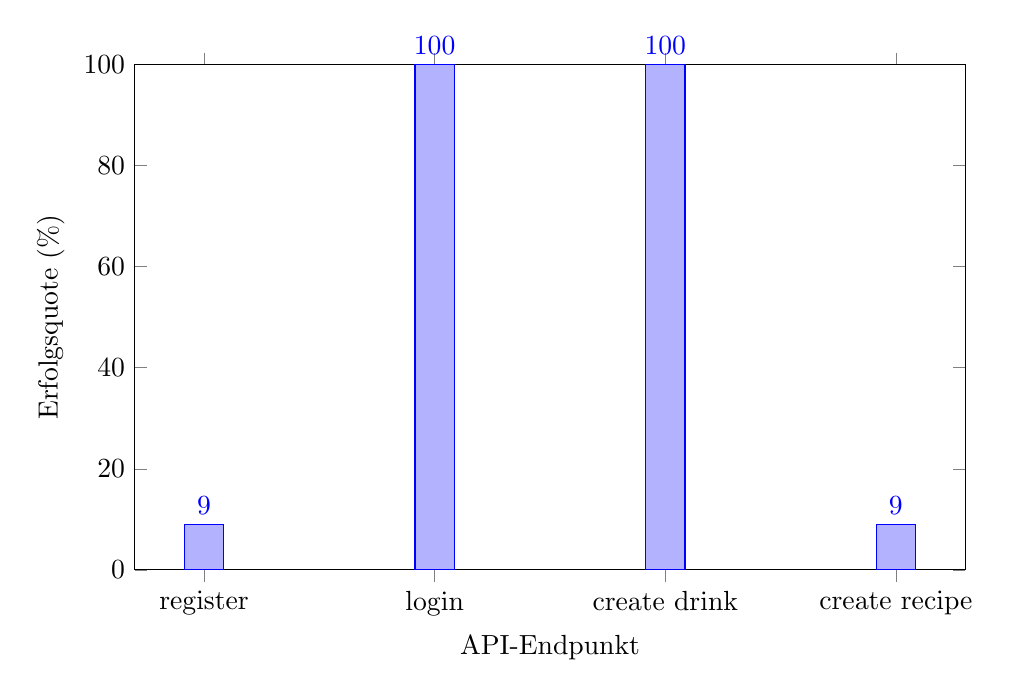
\begin{tikzpicture}
        \begin{axis}[
            ybar,
            width=\textwidth,
            height=8cm,
            xlabel={API-Endpunkt},
            ylabel={Erfolgsquote (\%)},
            ymin=0, ymax=100,
            symbolic x coords={register, login, create drink, create recipe},
            xtick=data,
            bar width=0.5cm,
            nodes near coords,
            nodes near coords align={vertical},
            ]
            \addplot coordinates {(register, 9) (login, 100) (create drink, 100) (create recipe, 9)};
        \end{axis}
    \end{tikzpicture}
    \caption{Erfolgsquoten der Haupt-API-Endpunkte}
    \label{fig:success_rates}
\end{figure}

\subsection*{Fehlerrate über die Zeit}
\begin{figure}
    \centering
    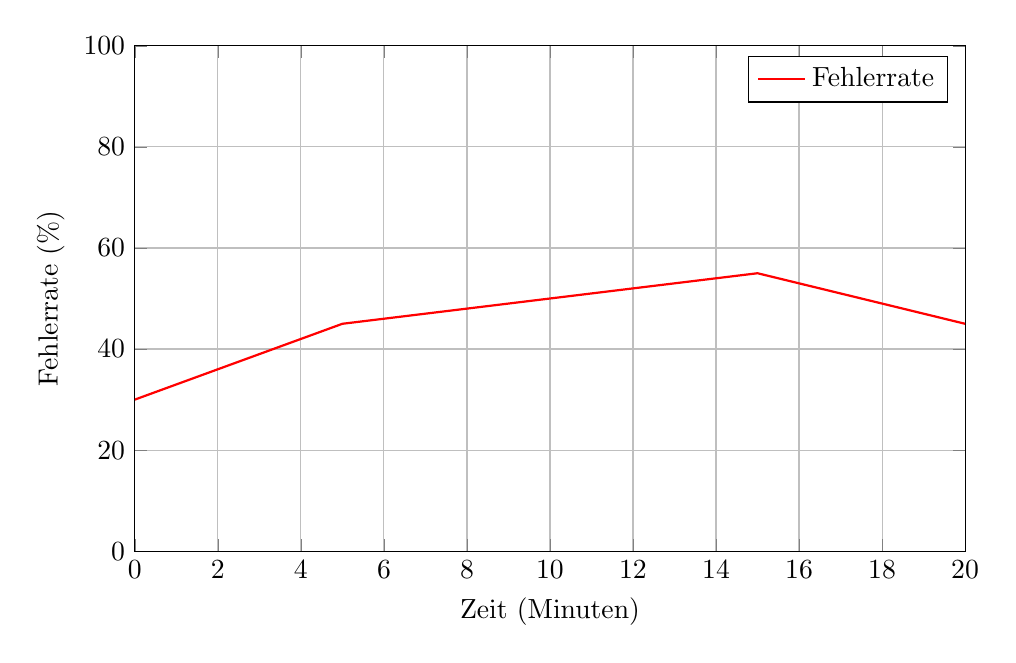
\begin{tikzpicture}
        \begin{axis}[
            width=\textwidth,
            height=8cm,
            xlabel={Zeit (Minuten)},
            ylabel={Fehlerrate (\%)},
            xmin=0, xmax=20,
            ymin=0, ymax=100,
            grid=both,
            ]
            \addplot[red, thick] coordinates {
                (0, 30) (5, 45) (10, 50) (15, 55) (20, 45)
            };
            \addlegendentry{Fehlerrate}
        \end{axis}
    \end{tikzpicture}
    \caption{Fehlerrate im Verlauf des Tests}
    \label{fig:error_rate}
\end{figure}

\section*{Schlussfolgerungen}
Die Ergebnisse zeigen, dass:
\begin{itemize}
    \item Die Benutzerregistrierung und Rezeptverwaltung besonders fehleranfällig sind (nur 9\% Erfolgsquote).
    \item Die API insgesamt eine hohe Fehlerrate von 45,11\% aufweist, was auf Skalierungs- oder Ressourcenprobleme hindeuten könnte.
    \item Die durchschnittliche Antwortzeit (66,26 ms) akzeptabel ist, aber in Spitzenzeiten (max. 644 ms) stark ansteigt.
\end{itemize}

\section*{Empfehlungen}
\begin{itemize}
    \item Optimieren Sie die Ressourcen- und Skalierungseinstellungen von Google Cloud Run.
    \item Reduzieren Sie die Last in der Benutzerregistrierung durch bessere Datenbankabfragen oder asynchrone Prozesse.
    \item Testen Sie kleinere Benutzergruppen, um die Schwellenwerte für Stabilitätsprobleme zu identifizieren.
\end{itemize}